\documentclass[a4paper,13pt]{article}
\setcounter{secnumdepth}{-1} 

\usepackage{amsmath}
\usepackage{amssymb}
\usepackage{courier}
\usepackage{graphicx}
\usepackage[utf8]{inputenc}

\usepackage[top=2cm, bottom=1cm, left=1.5cm, right=1.5cm,landscape]{geometry}

\usepackage{multicol}
\setlength{\columnseprule}{.1pt}

\usepackage{fancyhdr}
\pagestyle{fancy}
\lhead{Leandro Vianna [UFG]}
\rhead{\thepage}
\cfoot{}

\usepackage{color}
\definecolor{cstrings}{rgb}{0.6,0,0}
\definecolor{ccomments}{rgb}{0.25,0.5,0.35}
\definecolor{ckeywords}{rgb}{0.25,0.35,0.75}

\usepackage{listings}
\lstset{language=C++,
basicstyle=\scriptsize\ttfamily,
%keywordstyle=\color{ckeywords}\bfseries,
%stringstyle=\color{cstrings},
%commentstyle=\color{ccomments},
columns=fullflexible}

\newcommand\includefile[3]{
   \subsection{#1}
   \begin{multicols}{2}
    \lstinputlisting[language=c++]{#2/#3}
   \end{multicols}
}

\usepackage{datetime}

\begin{document}

\thispagestyle{fancy}
\begin{center}
	\Huge\textsc{Universidade Federal de Goiás \\ Team Reference Material}
	\
	
	\small \the\year{} South America/Brazil Regional Contest
\end{center}
\
\begin{multicols}{2}
\tableofcontents
\end{multicols}
\newpage

\includefile{Augmenting Path (MCBM)}{../lib}{augmenting_path.cpp}
\includefile{Combinations}{../lib}{combinations.cpp}
\includefile{Convex Hull}{../lib}{convex_hull.cpp}
\includefile{Debug Msg}{../lib}{debug_msg.cpp}
\includefile{Dinic (Max Flow)}{../lib}{dinic.cpp}
\includefile{Edmonds-Karp (Max Flow)}{../lib}{max_flow.cpp}
\includefile{Euler's Tour}{../lib}{euler_tour.cpp}
\includefile{Extended Euclids}{../lib}{extended_euclids.cpp}
\includefile{Fenwick Tree}{../lib}{fenwick.cpp}
\includefile{Fenwick Tree 2D}{../lib}{fenwick2d.cpp}
\includefile{Fenwick Tree 2D of XOR}{../lib}{fenwick2d_xor.cpp}
\includefile{Floyd Warshall}{../lib}{floyd_warshall.cpp}
\includefile{Gaussian Elimination}{../lib}{gaussian_elimination.cpp}
\includefile{Gaussian Elimination Xor}{../lib}{gaussian_elimination_xor.cpp}
\includefile{Generate Combinations}{../lib}{gen_combinations.cpp}
\includefile{Geometry}{../lib}{geometry.cpp}
\includefile{Geometry CP3}{../lib}{geometry_cp3.cpp}
\includefile{Getchar Unlocked}{../lib}{getchar_unlocked.cpp}
\includefile{Grundy Number}{../lib}{grundy_number.cpp}
\includefile{Kruskal (Minimum Spanning Tree)}{../lib}{kruskal.cpp}
\includefile{Lowest Common Ancestor (LCA)}{../lib}{lca.cpp}
\includefile{Longest Increasing Sequence}{../lib}{lis.cpp}
\includefile{Longest Increasing Sequence with Fenwick Tree}{../lib}{lis_fenwick.cpp}
\includefile{Longest Increasing Sequence (Print elements)}{../lib}{lis_print.cpp}
\includefile{Matrix Power}{../lib}{matrix_power.cpp}
\includefile{Minimum Cost Maximum Flow}{../lib}{min_cost_max_flow.cpp}
\includefile{Mo's Algorithm}{../lib}{mo.cpp}
\includefile{Ordered Set}{../lib}{ordered_set.cpp}
\includefile{Random Numbers}{../lib}{random_numbers.cpp}
\includefile{Rotating Calipers (Diameter of a polygon)}{../lib}{rotating_calipers.cpp}
\includefile{Strongly Connected Components (SCC)}{../lib}{scc.cpp}
\includefile{Sieve}{../lib}{sieve.cpp}
\includefile{String Hashing}{../lib}{string_hash.cpp}
\includefile{Suffix Array}{../lib}{suffix_array_n.cpp}
\includefile{Suffix Automata}{../lib}{suffix_automata.cpp}
\includefile{Topological Sort}{../lib}{topological_sort.cpp}
\includefile{Union Find}{../lib}{union_find.cpp}

\subsection{Suffix Automata's Applications}
Problem: Find whether a given string w is a substring of s.\\
Solution: Simply run the automaton.
\begin{verbatim}
SuffixAutomaton a(s);
bool fail = false;
int n = 0;
for(int i=0;i<w.size();i++) {
  if(a.edges[n].find(w[i]) == a.edges[n].end()) {
    fail = true;
    break;
  }
  n = a.edges[n][w[i]];
}
if(!fail) cout << w << " is a substring of " << s << "\n";
\end{verbatim}

Problem: Find whether a given string w is a suffix of s.\\
Solution: Construct the list of terminal states, run the automaton as above and check in the end if the n is among the terminal states.
Let's now look at the dp problems.

Problem: Count the number of distinct substrings in s.\\
Solution: The number of distinct substrings is the number of different paths in the automaton. These can be calculated recursively by calculating for each node the number of different paths starting from that node. The number of different paths starting from a node is the sum of the corresponding numbers of its direct successors, plus 1 corresponding to the path that does not leave the node.

Problem: Count the number of times a given word w occurs in s.\\
Solution: Similar to the previous problem. Let p be the node in the automaton that we end up while running it for w. This time the number of times a given word occurs is the number of paths starting from p and ending in a terminal node, so one can calculate recursively the number of paths from each node ending in a terminal node.

Problem: Find where a given word w occurs for the first time in s.\\
Solution: This is equivalent to calculating the longest path in the automaton after reaching the node p (defined as in the previous solution).

Finally let's consider the following problem where the suffix links come handy.

Problem: Find all the positions where a given word w occurs in s.\\
Solution: Prepend the string with some symbol '\$' that does not occur in the string and construct the suffix automaton. Let's then add to each node of the suffix automaton its children in the suffix tree:

\begin{verbatim}
children=vector<vector<int>>(link.size());
for(int i=0;i<link.size();i++) {
  if(link[i] >= 0) children[link[i]].push_back(i);
}
\end{verbatim}

Now find the node p corresponding to the node w as has been done in the previous problems. We can then dfs through the subtree of the suffix tree rooted at p by using the children vector. Once we reach a leaf, we know that we have found a prefix of s that ends in w, and the length of the leaf can be used to calculate the position of w. All of the dfs branches correspond to different prefixes, so no unnecessary work is done and the complexity is $O(|s| + |w| + size of output)$.

\subsection{Combinatorics}
\subsubsection{Binomial Coefficients}

Number of ways to pick a multiset of sike $k$ from $n$ elements: $\binom{n+k-1}{k}$\\
Number of $n$-tuples of non-negative integers with sum $s$: $\binom{s+n-1}{n-1}$, at most $s$: $\binom{s+n}{n}$\\
Number of $n$-tuples of positive integers with sum $s$: $\binom{s-1}{n-1}$\\
Number of lattice paths from $(0,0)$ to $(a,b)$, restricted to east and north steps: $\binom{a+b}{a}$

$v_{r,c} = v_{r,c-1} \frac{r+1-c}{c}$

$x = r_0$; $y = 1$; $a_{r,c} = a_{r-1,c-1}  \frac{++x}{++y}, r \geq r_0+2, c \geq 2$

\subsubsection{Catalan numbers}
$C_{n} = \frac{1}{n+1}\binom{2n}{n}$. $C_0 = 1$,  $C_{n} = \sum_{i=0}^{n-1}C_iC_{n-1-i}$. $C_{n+1} = C_{n}\frac{4n+2}{n+2}$.\\
$C_0,C_1,... $ = 1, 1, 2, 5, 14, 42, 132, 429, 1430, 4862, 16796, 58786, 208012, 742900, ...\\
$C_{n}$ is the number of: properly nested sequences of $n$ pais of parentheses; rooted ordered binary trees with $n+1$ leaves; triangulations of a convex $(n+2)$-gon.

\subsubsection{Derangements}
Number of permutations of $n = 0,1,2,...$ elements without fixed points is 1, 0, 1, 2, 9, 44, 265, 1854, 14833, ... Recurrence: $D_{n} = (n-1)(D_{n-1} + D_{n-2}) = nD_{n-1} + (-1)^{n}$.
Corollary: number of permutations with exactly $k$ fixed points is $\binom{n}{k}D_{n-k}$.

\subsubsection{Bell numbers}
$B_{n}$ is the number of partitions of $n$ elements. $B_0$, ... = 1, 1, 2, 5, 15, 52, 203, ...\\
$B_{n+1} = \sum_{k=0}^{n}\binom{n}{k}B_{k} = \sum_{k=1}^{n} S_{n,k}$. Bell triangle: $B_r = a_{r,1} = a_{r-1,r-1}, a_{r,c} = a_{r-1,c-1} + a_{r,c-1}$.

\subsubsection{Eulerian numbers}
$E(n, k)$ is the number of permutations with exactly $k$ descents $(i : \pi_{i} < \pi_{i+1})$ / ascents $(\pi_{i} > \pi_{i+1})$ / excedances $(\pi_{i} > i)$ / $k + 1$ weak excedances $(\pi_{i} \geq i)$.\\
Formula: $E(n,k) = (k+1)E(n-1,k) + (n-k)E(n-1,k-1)$.

\subsubsection{Burnside's lemma}
The number of orbits under $G$'s action on set $X$ : $|X/G| = \frac{1}{|G|} \sum_{g \in G} |X_g|$, where $X_g = \{x \in X : g(x) = x\}$. (``Average number of fixed points.'')
Let $w(x)$ be weight of $x$'s orbit. Sum of all orbits' weights: $\sum_{o \in X/G}w(o) = \frac{1}{|G|} \sum_{g \in G} \sum_{x \in X_g} w(x)$.

\subsection{Number Theory}
\subsubsection{Linear diophantine equation}
$ax + by = c$. Let $d = gcd(a,b)$. A solution exists iff $d|c$. If $(x_0, y_0)$ is any solution, then all solutions are given by $(x, y) = (x_0 + \frac{b}{d}t, y_0 - \frac{a}{d}t), t \in \mathbb{Z}$. To find some solution $(x_0, y_0)$,
use extended GCD to solve $ax_0 + by_0 = d = gcd(a, b)$, and multiply its solutions by $\frac{c}{d}$.\\
Linear diophantine equation in $n$ variables: $a_1x_1 + ... + a_nx_n = c$ has solutions iff $gcd(a_1, ..., a_n) | c$. To find some solution, let $b = gcd(a_2, ..., a_n)$, solve $a_1x_1 + by = c$, and iterate with $a_2x_2 + ... = y$.

$a^{-1} (mod\ n) = a^{\phi(n)-1}$

$n\ prime \rightarrow a^{-1} (mod\ n) = a^{n-2}$

\subsubsection{Chinese Remainder Theorem}
System $x \equiv a_i (mod\ m_i)$ for $i = 1, ..., n$ with pairwise relatively prime $m_i$ has a unique solution modulo $M = m_1m_2...m_n : x = a_1b_1\frac{M}{m_1} + ... + a_nb_n\frac{M}{m_n} (mod\ M)$, where $b_i$ is modular inverse of $\frac{M}{M_i}$ modulo $m_i$.\\
System $x \equiv a (mod\ m), x \equiv b (mod\ n)$ has solutions iff $a \equiv b (mod\ g)$, where $g = gcd(m,n)$. The solution is unique modulo $L = \frac{mn}{g}$, and equals: $x \equiv a + T(b-a)m/g \equiv b + S(a-b)n/g (mod\ L)$, where $S$ and $T$ are integer solutions of $mT + nS = gcd(m,n)$.

\subsubsection{Prime-counting function}
$\pi(n) = |\{p \leq n : p\ is\ prime\}|$. $n / ln(n) < \pi(n) < 1.3n / ln(n)$. $\pi(1000) = 168, \pi(10^6) = 78498, \pi(10^9) = 50 847 534$. $n$-th prime $\approx n ln(n)$.

\subsubsection{Miller-Rabin's primality test}
Given $n = 2^{r}s + 1$ with odd s, and a random integer $1 < a < n$. If $a^{s} \equiv 1 (mod\ n)$ or $a^{2^{j}s} \equiv -1 (mod\ n)$ for some $0 \leq j \leq r-1$, then $n$ is a probable prime.

\subsubsection{Pollard-$\rho$}
Choose random $x_1$, and let $x_{i+1} = x_{i}^{2} (mod\ n)$. Test $gcd(n,x_{2^k+i} - x_{2^k})$ as possible $n$'s factors for $k = 0, 1, ...$ Expected time to find a factor: $O(\sqrt{m})$, where $m$ is smallest prime power in $n$'s factorization. That's $O(n^{1/4})$ if you check $n = p^k$ as a special case before factorization.

\subsubsection{Fermat primes}
A Fermat prime is a prime of form $2^{2^n} + 1$. The only known Fermat primes are 3, 5, 17, 257, 65537. A number of form $2^{n} + 1$ is prime only if it is a Fermat prime.

\subsubsection{Perfect numbers}
$n > 1$ is called perfect if it equals sum of its proper divisors and 1. Even $n$ is perfect iff $n = 2^{p-1}(2^{p} - 1)$ and $2^{p} - 1$ is prime (Mersenne’s). No odd perfect numbers are yet found.

\subsubsection{Carmichael numbers}
A positive composite $n$ is a Carmichael number $(a^{n-1} \equiv 1 (mod\ n)$ for all $a: gcd(a,n) = 1)$, iff $n$ is square-free, and for all prime divisors $p$ of $n$, $p-1$ divides $n-1$.

\subsubsection{Number/sum of divisors}
$\tau(p_1^{a_1}...p_k^{a_k}) = \prod_{j=1}^{k}(a_j + 1).$

$\sigma(p_1^{a_1}...p_k^{a_k}) = \prod_{j=1}^{k}\frac{p_{j}^{a_j+1}-1}{p_j-1}.$

\subsubsection{Euler's phi function}

$\phi(n) = |\{m \in \mathbb{N}, m \leq n, gcd(m,n) = 1\}|$.

$\phi(mn) = \frac{\phi(m)\phi(n)gcd(m,n)}{\phi(gcd(m,n))}$.

$\phi(p^a) = p^{a-1}(p-1)$.

$\sum_{d|n}\phi(d) = \sum_{d|n}\phi(\frac{n}{d}) = n$.

\subsubsection{Euler's Theorem} 
$a^{\phi(n)} \equiv 1 (mod\ n)$, if $gcd(a,n) = 1$.

\subsubsection{Wilson's Theorem} 
$p$ is prime iff $(p-1)! \equiv -1 (mod\ p)$

\subsubsection{Mobius function}
$\mu(1) = 1$.\\
$\mu(n) = 0$, if $n$ is not square free.\\
$\mu(n) = (-1)^{s}$, if $n$ is the product of s distinct primes.\\
Let $f$, $F$ be functions on positive integers. If for all $n \in \mathbb{N}$, $F(n) = \sum_{d|n}f(d)$, then $f(n) = \sum_{d|n}\mu(d)F(\frac{n}{d})$, and vice versa.\\
$\phi(n) = \sum_{d|n}\mu(d)\frac{n}{d}$.\\
$\sum_{d|n}\mu(d) = 1$.\\
If $f$ is multiplicative, then $\sum_{d|n}\mu(d)f(d) = \prod_{p|n}(1-f(p))$, $\sum_{d|n}\mu(d)^2f(d) = \prod_{p|n}(1+f(p))$\\
f[i] = 1, f[p] = -1, f[j] *= (j\%(i*i)==0)? 0 : -1;

\subsubsection{Legendre symbol}
If $p$ is an odd prime, $a \in \mathbb{Z}$, then $(\frac{a}{p})$ equals 0, if $p|a$; 1 if $a$ is a quadratic residue modulo $p$; and -1 otherwise. Euler's criterion: $(\frac{a}{p}) = a^{(\frac{p-1}{2})} (mod\ p)$.

\subsubsection{Jacobi symbol}
If $n = p_1^{a_1}...p_k^{a_k}$ is odd, then $(\frac{a}{n}) = \prod_{i=1}^k(\frac{a}{p_i})^{k_i}$.

\subsubsection{Primitive roots}
If the order of $g$ modulo $m$ (min $n > 0: g^n \equiv 1 (mod\ m))$ is $\phi(m)$, then $g$ is called a primitive root.
If $\mathbb{Z}_m$ has a primitive root, then it has $\phi(\phi(m))$ distinct primitive roots.
$\mathbb{Z}_m$ has a primitive root iff $m$ is one of $2, 4, p^k, 2p^k$, where $p$ is an odd prime. If $\mathbb{Z}_m$ has a primitive root $g$, then for all $a$ coprime to $m$, there exists unique integer $i = ind_g(a)$ modulo $\phi(m)$,
such that $g^i \equiv a (mod\ m)$. $ind_g(a)$ has logarithm-like properties: $ind(1) = 0$, $ind(ab) = ind(a) + ind(b)$.\\
If $p$ is prime and $a$ is not divisible by $p$, then congruence $x^n \equiv a (mod\ p)$ has $gcd(n, p - 1)$ solutions if $a^{(p-1)/ gcd(n,p-1)} \equiv 1 (mod\ p)$, and no solutions otherwise.

\subsubsection{Discrete log}
Find $x$ from $a^x \equiv b (mod\ m)$. Can be solved in $O(\sqrt{m})$ time and space with a meet-in-the-middle trick. Let $n = \lceil \sqrt{m} \rceil$, and $x = ny - z$. Equation becomes $a^{ny} \equiv ba^z (mod\ m)$.
Precompute all values that the RHS can take for $z$ = 0,1,...,n-1, and brute force y on the LHS, each time checking whether there’s a corresponding value for RHS.

\subsubsection{Pythagorean triples}
Integer solutions of $x^2 + y^2 = z^2$. All relatively prime triples are given by: $x = 2mn, y = m^2 - n^2, z = m^2 + n^2$ where $m > n$, $gcd(m,n) = 1$ and $m \not\equiv n (mod\ 2)$. All other triples
are multiples of these. Equation $x^2 + y^2 = 2z^2$ is equivalent to $(\frac{x+y}{2})^2 + (\frac{x-y}{2})^2 = z^2$.

\subsubsection{Postage stamps/McNuggets problem}
Let $a, b$ be relatively-prime integers. There are exactly $\frac{1}{2}(a-1)(b-1)$ numbers \emph{not} of form $ax + by (x,y \geq 0)$, and the largest is $(a-1)(b-1)-1 = ab-a-b$.

\subsubsection{Fermat's two-squares theorem}
Odd prime $p$ can be represented as a sum of two squares iff $p \equiv 1 (mod\ 4)$. A product of two sums of two squares is a sum of two squares. Thus, $n$ is a sum of two squares iff every prime of form $p = 4k + 3$ occurs an even number of times in $n$'s factorization.

\subsection{Graphs}
\subsubsection{Euler’s theorem}
For any planar graph, $V - E + F = 1 + C$, where $V$ is the number of graph’s vertices, $E$ is the number of edges, $F$ is the number of faces in graph’s planar drawing,
and $C$ is the number of connected components. Corollary: $V - E + F = 2$ for a 3D polyhedron.

\subsubsection{Vertex covers and independent sets}
Let $M$, $C$, $I$ be a max matching, a min vertex cover, and a max independent set. Then $|M| \leq |C| = N - |I|$, with equality for bipartite graphs. Complement of an MVC is always a MIS, and vice versa.
Given a bipartite graph with partitions $(A,B)$, build a network: connect source to $A$, and $B$ to sink with edges of capacities, equal to the corresponding nodes’ weights, or 1 in the unweighted case.
Set capacities of the original graph’s edges to the infinity. Let $(S,T)$ be a minimum $s-t$ cut. 
Then a maximum(-weighted) independent set is $I = (A \bigcap S) \bigcup (B \bigcap T)$, and a minimum(-weighted) vertex cover is $C = (A \bigcap T) \bigcup (B \bigcap S)$.

\subsubsection{Matrix-tree theorem}
Let matrix $T = [t_{ij}]$, where $t_{ij}$ is the number of multiedges between $i$ and $j$, for $i \neq j$, and $t_{ii} = -deg_i$.
Number of spanning trees of a graph is equal to the determinant of a matrix obtained by deleting any $k$-th row and $k$-th column from $T$.

\subsubsection{Prufer code of a tree}
Label vertices with integers 1 to $n$. Repeatedly remove the leaf with the smallest label, and output its only neighbor’s label, until only one edge remains. The sequence has length $n - 2$.
Two isomorphic trees have the same sequence, and every sequence of integers from 1 and $n$ corresponds to a tree. Corollary: the number of labelled trees with $n$ vertices is $n^{n-2}$.

\subsubsection{Euler tours}
Euler tour in an undirected graph exists iff the graph is connected and each vertex has an even degree. Euler tour in a directed graph exists iff in-degree of each vertex equals its out-degree, and underlying undirected graph is connected.

\subsubsection{Stable marriage problem}
While there is a free man $m$: let $w$ be the most-preferred woman to whom he has not yet proposed, and propose $m$ to $w$. If $w$ is free, or is engaged to someone whom she prefers less than $m$, match $m$ with $w$, else deny proposal.

%\subsubsection{Stoer-Wagner}
\includefile{Stoer-Wagner}{../lib}{stoer_wagner.cpp}
Start from a set $A$ containing an arbitrary vertex. While $A \neq V$, add to $A$ the most tightly connected vertex ($z \not\in A$ such that $\sum_{x\in A}w(x,z)$ is maximized.)
Store cut-of-the-phase (the cut between the last added vertex and rest of the graph), and merge the two vertices added last. Repeat until the graph is contracted to a single vertex. Minimum cut is one of the cuts-of-the-phase.

\subsubsection{Erdos-Gallai theorem}
A sequence of integers $\{d_1,d_2,...,d_n\}$, with $n-1 \geq d_1 \geq d_2 \geq ... \geq d_n \geq 0$ is a degree sequence of some undirected simple graph iff $\sum d_i$ is even and $d_1+ ... + dk \leq k(k-1)+ \sum_{i=k+1}^{n}min(k, d_i)$
for all $k = 1, 2, . . . , n - 1$.

\subsubsection{Dilworth's theorem}
In any finite partially ordered set, the maximum number of elements in any antichain equals the minimum number of chains in any partition of the set into chains.

Dilworth's theorem characterizes the width of any finite partially ordered set in terms of a partition of the order into a minimum number of chains.\\
An antichain in a partially ordered set is a set of elements no two of which are comparable to each other, and a chain is a set of elements every two of which are comparable. Dilworth's theorem states that there exists an antichain $A$,
and a partition of the order into a family $P$ of chains, such that the number of chains in the partition equals the cardinality of $A$. When this occurs, $A$ must be the largest antichain in the order, for any antichain can have at most one
element from each member of $P$. Similarly, $P$ must be the smallest family of chains into which the order can be partitioned, for any partition into chains must have at least one chain per element of $A$. The width of the partial order is
defined as the common size of $A$ and $P$.

\subsection{Games}
\subsubsection{Grundy numbers}
For a two-player, normal-play (last to move wins) game on a graph ($V,E$): $G(x)=mex(\{G(y) : (x,y) \in E\})$, where $mex(S)=min\{n \geq 0 : n \not\in S\}$. $x$ is losing iff $G(x)=0$.

\subsubsection{Sums of games}
\begin{itemize}
\item Player chooses a game and makes a move in it. Grundy number of a position is xor of grundy numbers of positions in summed games.
\item Player chooses a non-empty subset of games (possibly, all) and makes moves in all of them. A position is losing iff each game is in a losing position.
\item Player chooses a proper subset of games (not empty and not all), and makes moves in all chosen ones. A position is losing iff grundy numbers of all games are equal.
\item Player must move in all games, and loses if can’t move in some game. A position is losing if any of the games is in a losing position.
\end{itemize}

\subsubsection{Misère Nim}
A position with pile sizes $a_1,a_2,...,a_n \geq 1$, not all equal to 1, is losing iff $a_1 \bigoplus a_2 \bigoplus ... \bigoplus a_n = 0$ (like in normal nim.)
A position with $n$ piles of size 1 is losing iff $n$ is odd.

\subsection{Geometry}

\subsubsection{Pick's theorem}
$I = A - B/2 + 1$, where $A$ is the area of a lattice polygon, $I$ is the number of lattice points inside it, and $B$ is the number of lattice points on the boundary. Number of lattice points minus one on a line segment from (0, 0) and (x, y) is gcd(x, y).

\bigskip

$a . b = a_{x}b_{x} + a_{y}b_{y} = |a| . |b| . cos(\theta)$

$a \times b = a_{x}b_{y} - a_{y}b_{x} = |a| . |b| . sin(\theta)$

3D: $a \times b = (a_{y}b_{z} - a_{z}b_{y}, a_{z}b_{x} - a_{x}b_{z}, a_{x}b_{y} - a_{y}b_{x})$

\subsubsection{Line}
Line $ax + by = c$ through $A(x_{1}, y_{1})$ and $B(x_{2}, y_{2})$: $a = y_{1} - y_{2}$, $c = x_{2} - x_{1}$, $c = ax_{1} + by_{1}$.\\
Half-plane to the left of the directed segment $AB$: $ax + by \geq c$.\\
Normal vector: $(a, b)$. Direction vector: $(b, -a)$. Perpendicular line: $-bx + ay = d$.\\
Point of intersection of $a_{1}x + b_{1}y = c_{1}$ and $a_{2}x + b_{2}y = c_{2}$ is $\frac{1}{a_{1}b_{2} - a_{2}b_{1}}(c_{1}b_{2} - c_{2}b_{1}, a_{1}c_{2} - a_{2}c_{1})$.\\
Distance from line $ax + by + c = 0$ to point $(x_{0}, y_{0})$ is $|ax_{0} + by_{0} + c|/\sqrt{a^2 + b^2}$.\\
Distance from line AB to P (for any dimension): $\frac{|(A - P) \times (B - P)|}{|A - B|}$.\\
Point-line segment distance:

if $(dot(B - A, P - A) < 0)$ return $dist(A, P);$

if $(dot(A - B, P - B) < 0)$ return $dist(B, P);$

return $fabs(cross(P, A, B)/dist(A, B));$

\subsubsection{Projection}
Projection of point $C$ onto line $AB$ is $\frac{AB.AC}{AB.AB}AB$.\\
Projection of $(x_{0}, y_{0})$ onto line $ax + by = c$ is $(x_{0}, y_{0}) + \frac{1}{a^2 + b^2}(ad, bd)$, where $d = c - ax_{0} - by_{0}$.\\
Projection of the origin is $\frac{1}{a^2 + b^2}(ac, bc)$.

\subsubsection{Segment-segment intersection}
Two line segments intersect if one of them contains an endpoint of the other segment, or each segment straddles the line, containing the other segment ($AB$ straddles line $l$ if $A$ and $B$ are on the opposite sides of $l$.)

\subsubsection{Circle-circle and circle-line intersection}
 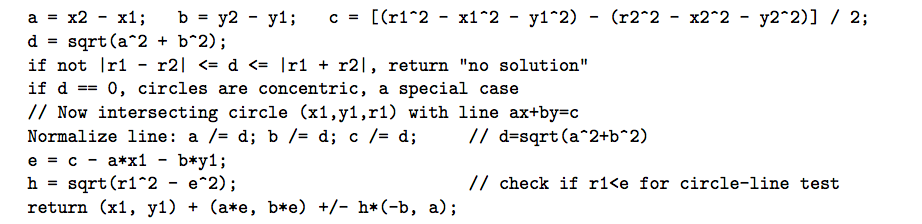
\includegraphics[scale=.7]{../lib/candc.png}

\subsubsection{Circle from 3 points (circumcircle)}
Intersect two perpendicular bisectors. Line perpendicular to $ax + by = c$ has the form $-bx + ay = d$. Find $d$ by substituting midpoint’s coordinates.

\subsubsection{Angular bisector}
Angular bisector of angle $ABC$ is line $BD$, where $D = \frac{BA}{|BA|} + \frac{BC}{|BC|}$.\\
Center of incircle of triangle $ABC$ is at the intersection of angular bisectors, and is $\frac{a}{a+b+c}A + \frac{b}{a+b+c}B + \frac{c}{a+b+c}C$
where $a$, $b$, $c$ are lengths of sides, opposite to vertices $A$, $B$, $C$. Radius $= \frac{2S}{a+b+c}$

\subsubsection{Counter-clockwise rotation around the origin}
$(x,y) \rightarrow (x\cos\phi - y\sin\phi, x \sin\phi + y \cos\phi)$.\\
90-degrees counter-clockwise rotation: $(x,y) \rightarrow (-y,x)$. Clockwise: $(x,y) \rightarrow (y,-x)$.

\subsubsection{3D rotation}
3D rotation by ccw angle $\phi$ around axis $n$: $r' = r \cos\phi + n(n \cdot r)(1 - \cos \phi) + (n \times r) \sin\phi$

\subsubsection{Plane equation from 3 points}
$N \cdot (x, y, z) = N \cdot A$, where $N$ is normal: $N = (B - A) \times (C - A)$.

\subsubsection{3D figures}
Sphere: Volume $V = \frac{4}{3}\pi r^3$, surface area $S = 4\pi r^2$

$x = \rho \sin \theta \cos\phi$, $y = \rho \sin\theta\sin\phi$, $z = \rho\cos\theta$, $\phi \in [-\pi,\pi], \theta \in [0,\pi]$\\
Spherical section: Volume $V = \pi h^2(r - h/3)$, surface area $S = 2\pi rh$\\
Pyramid: Volume $V = \frac{1}{3}h S_{base}$\\
Cone: Volume $V = \frac{1}{3} \pi r^2h$, lateral surface area $S = \pi r \sqrt{r^2 + h^2}$

\subsubsection{Area of a simple polygon}
$\frac{1}{2}\sum_{i=0}^{n-1}(x_iy_{i+1} - x_{i+1}y_i)$, where $x_n = x_0$, $y_n = y_0$.
Area is negative if the boundary is oriented clockwise.

\subsubsection{Winding number}
Shoot a ray from given point in an arbitrary direction. For each intersection of ray with polygon’s side, add +1 if the side crosses it counterclockwise, and -1 if clockwise.

%\includefile{Range Tree}{../lib/geometry}{range_tree.cpp}
%\includefile{KD Tree}{../lib/geometry}{kd_tree.cpp}
%\includefile{Enclosing Circle}{../lib/geometry}{enclosing_circle.cpp}
%
%\includefile{Geometry Basics}{../lib/geometry}{geobasics.cpp}
%\includefile{3D Geometry Basics}{../lib/geometry}{3dbasics.cpp}
%\includefile{Polygon Basics}{../lib/geometry}{pbasics.cpp}
%\includefile{Plane and Operations}{../lib/geometry}{pops.cpp}
%\includefile{Intersections}{../lib/geometry}{intersections.cpp}
%
%\includefile{Angles}{../lib/geometry}{angles.cpp}
%\includefile{Triangles}{../lib/geometry}{triangles.cpp}
%\includefile{Grate Circle Distance}{../lib/geometry}{grtcrcldist.cpp}
%
%\includefile{Convex Hull (Line Sweep)}{../lib/geometry}{hull_ls.cpp}
%\includefile{Graham Scan}{../lib/geometry}{gscan.cpp}
%\includefile{Circles Intersections}{../lib/geometry}{cintersect.cpp}
%\includefile{Closest Point}{../lib/geometry}{clstpnt.cpp}
%\includefile{Closest Points and Distances 3D}{../lib/geometry}{clstpnt3d.cpp}
%\includefile{Line Sweep Applications}{../lib/geometry}{line_sweep.cpp}


\end{document}
